\documentclass{beamer}
%[aspectratio=169]   \usepackage[czech]{babel}
\usepackage{apo-lecture}
\usepackage{pdfpages}
\usepackage{pdfcomment}
\usepackage{listings}
\usepackage{array,multirow}

\subtitle{Lekce 01. Úvod}
\author{Petr Štěpán\\ \small\texttt{stepan@fel.cvut.cz}}
\begin{document}

\maketitle

\section{Úvod}


\begin{frame}
\frametitle{Motivace}
Co ovlivňuje rychlost vykonávání Vašich programů:
\begin{itemize}
\item Výkon CPU 
  \begin{itemize}
    \item Frekvence CPU
    \item Efektivita CPU - kolik operací stihne provést za 1 takt procesoru
    \item Efektivita načítání dat z paměti
  \end{itemize}
\item Počet jader CPU
  \begin{itemize}
    \item Lze Váš program paralelizovat?
    \item Pokud ne, pak je jedno, kolik jader má CPU
    \item I pokud ano, tak nikdy nejde paralelizovat celý výpočet
  \end{itemize}
\end{itemize}
\end{frame}


\begin{frame}
\frametitle{Motivace}
Proč studovat architektury počítačů:
\begin{itemize}
\item Poptávka po absolventech kombinující umělou inteligenci a vestavné systémy (embedded system)
\item Pokud je pro Vás počítač BlackBox, pak jsou Vaše programy neefektivní
\item Pokud je Váš program pomalý neefektivní, nesplňuje kritéria např. pro rychlost řízení, pak máte několik možností:
\begin{itemize}
  \item zjistit, v čem současný počítač zpomaluje výpočet (rychlost procesoru, velikost vyrovnávací paměti, latence hlavní paměti, počet výpočetních jader) a otestovat jiný HW
  \item zjistit, zda lze program upravit, aby využíval lépe dostupné prostředky 
  \begin{itemize}
    \item upravit pořadí přístupu do paměti a tím lépe využíval vyrovnávací paměť
    \item upravit program, aby požíval méně skoků a tím se vykonával rychleji
    \item paralelizovat výpočet, využít specializovaný HW - GPU, externí výpočetní jednotku např. Coral USB nebo Intel Neural Compute Stick 2.
  \end{itemize}
\end{itemize}
\end{itemize}
\end{frame}


\begin{frame}
\frametitle{Obsah přednášek}
Projdeme si všechny základní součásti počítače:
\begin{itemize}
\item CPU
\item Hierarchie paměti - Cache/RAM
\item Vstupy a výstupy - I/O
\item Výjimky a přerušení
\end{itemize}
\end{frame}

\begin{frame}
\frametitle{Náplň cvičení}

\begin{columns}
\begin{column}{0.6\textwidth}
\begin{itemize}
\item 4 menší domácí úkoly - 36 bodů
\begin{itemize}
\item 2 programy v C
\item 2 formuláře
\item alespoň 3 úlohy ze 4
\end{itemize}
\item Semestrální úloha - 24 bodů
\begin{itemize}
\item Týmový projekt - dvojice, nebo jednotlivci
\item Speciální HW MZ APO deska
\end{itemize}
\end{itemize}
\end{column}
\begin{column}{0.35\textwidth}  
   \begin{tabular}{|l|l|}\hline
   Známka & Body\\ \hline
   A & >=90\\ \hline
   B & 80 -- 89.9\\ \hline
   C & 70 -- 79.9\\ \hline
   D & 60 -- 69.9\\ \hline
   E & 50 -- 59.9\\ \hline
   F & <50\\ \hline
   \end{tabular}
\end{column}
\end{columns}
\begin{itemize}
\item Nepoviné úlohy nebo aktivita při cvičení - 8 bodů
\end{itemize}
\bigskip
Zkouška: 
\begin{itemize}
\item písemný test 30 bodů, min 15 bodů
\item ústní $\pm$ 10 bodů    
\end{itemize}

\end{frame}


\begin{frame}
\frametitle{Navazující předměty}
Pokud Vás tento předmět zaujme, tak na něj navazují tyto předměty:
\begin{itemize}
\item B4M35PAP - Pokročilé architektury počítačů
\item B3B38VSY - Vestavné systémy
\item B4M38AVS - Aplikace vestavných systémů
\item B4B35OSY - Operační systémy
\item B0B35LSP - Logické systémy a procesory
\end{itemize}
\end{frame}


\begin{frame}
\frametitle{Materiály k předmětu}
\begin{itemize}
\item Paterson, D., Hennessey, V.: Computer Organization and Design, The HW/SW Interface. Elsevier, ISBN: 978-0-12-370606-5 (dostupná v knihovně FEL)
\item web:
\begin{itemize}
\item https://cw.fel.cvut.cz/b192/courses/b35apo/
\item https://dcenet.felk.cvut.cz/apo/
\end{itemize}
\item Kurzy v angličtině:
\begin{itemize}
\item MIT 6.004/6.191 – Computation Structures
\item Computation Structures | Electrical Engineering and Computer Science | MIT OpenCourseWare (2015)
\item Computer System Architecture | Electrical Engineering and Computer Science | MIT OpenCourseWare (2005)
\end{itemize}
\item Kurzy v češtině:
\begin{itemize}
\item https://courses.fit.cvut.cz/BI-APS/
\item https://www.vut.cz/studenti/predmety/detail/218515?apid=218515
\end{itemize}

\end{itemize}
\end{frame}

\section{Složení počítače}
\begin{frame}
\frametitle{Co je uvnitř počítače}

Základní deska počítače:
\begin{center}
   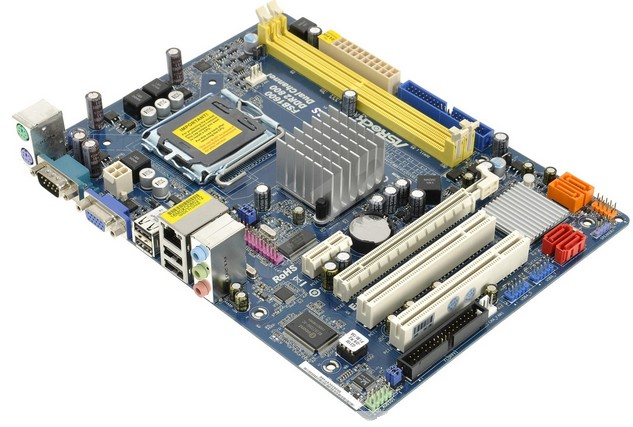
\includegraphics[width=0.8\textwidth]{fig/motherboard.jpg}
\end{center}

\end{frame}

\begin{frame}
\frametitle{Co je uvnitř počítače}

Rozebraný telefon:
\begin{center}
   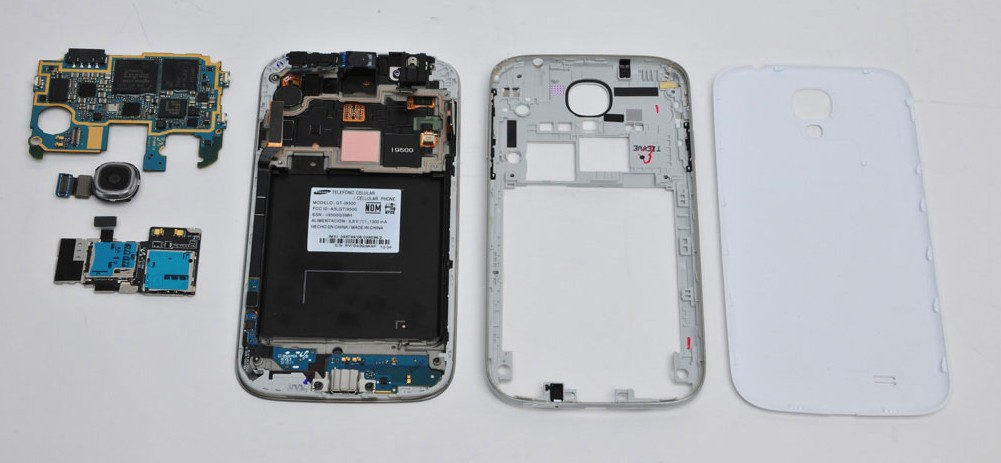
\includegraphics[width=0.6\textwidth]{fig/mobile.jpg}
\end{center}
\begin{center}
   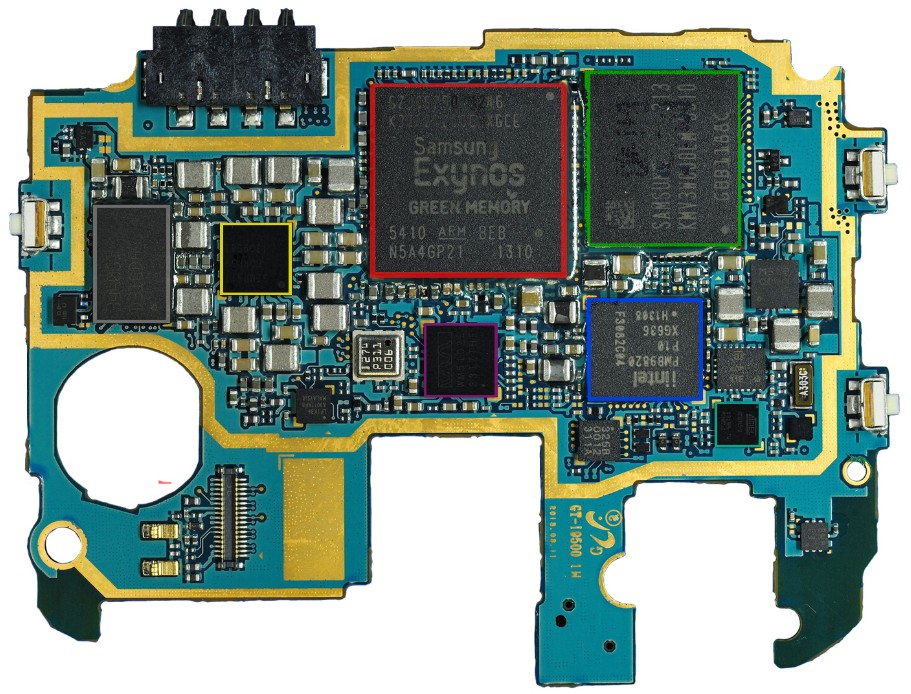
\includegraphics[width=0.4\textwidth]{fig/mobile-cpu.jpg}
\end{center}
\end{frame}


\begin{frame}
\frametitle{von Neumann}

Společný koncept navržený maďarským fyzikem Johnem von Neumannem (1903-1957) obsahuje:
\begin{itemize}
\item Procesor - Central Processing Unit - CPU
\item Paměť - Memory, Random-access Memory, 
\item Vstup/Výstup - Input/Output
\end{itemize}
\begin{center}
   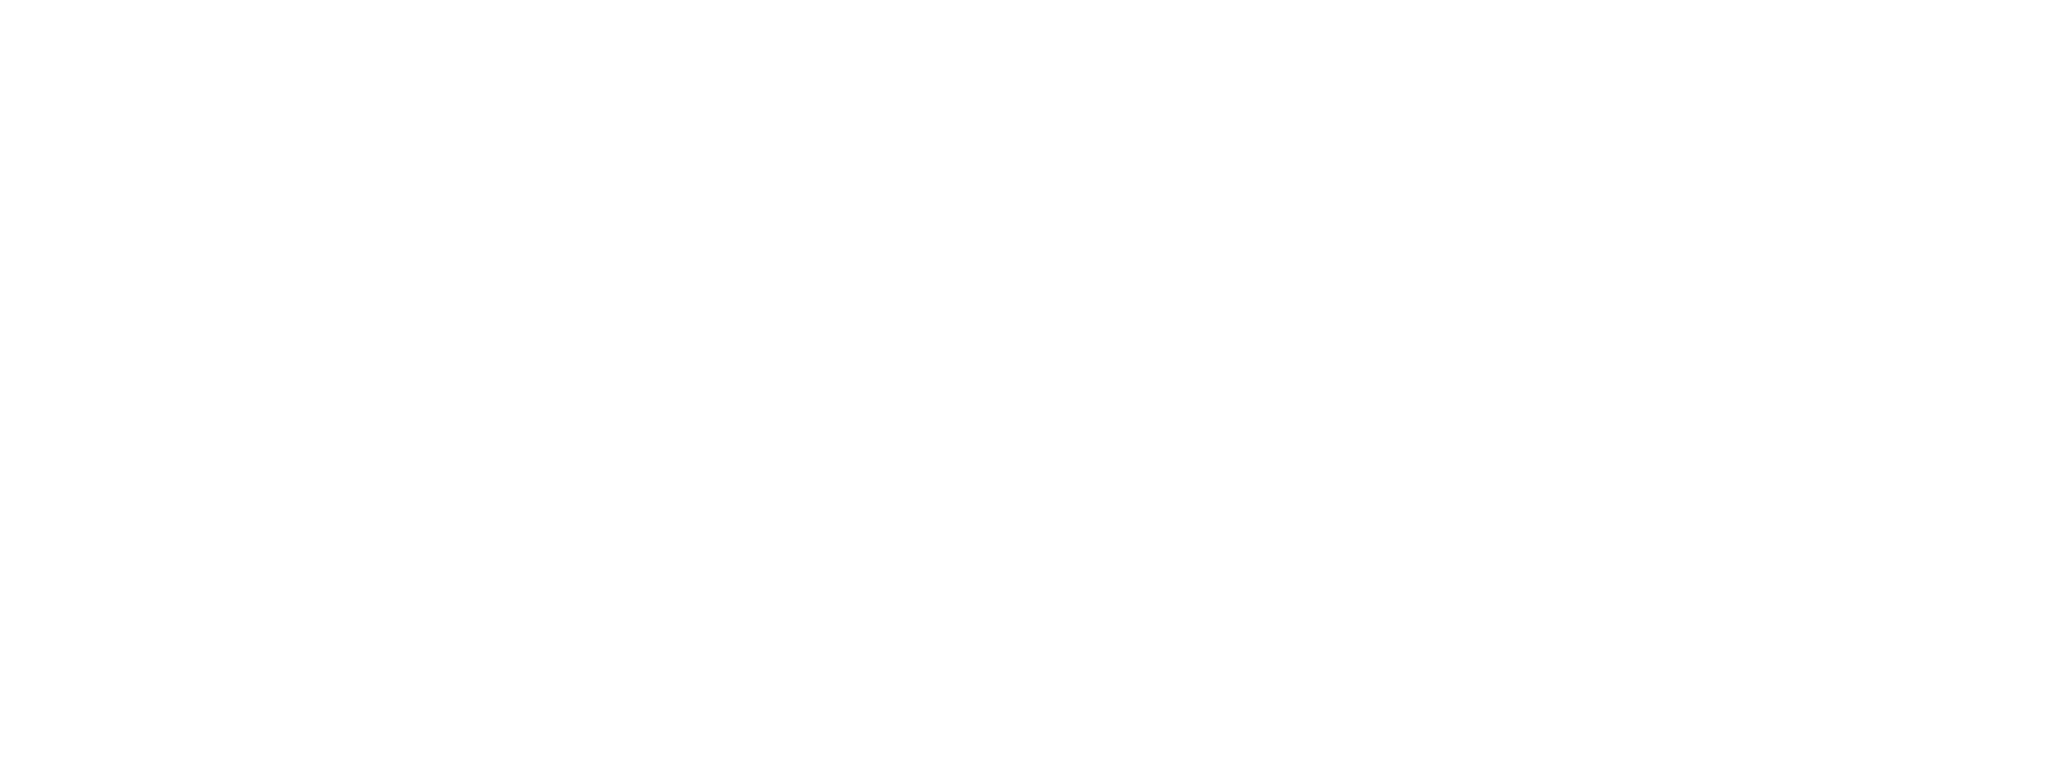
\includegraphics[width=0.7\textwidth]{cpu-vonNeumann.pdf}
\end{center}

\end{frame}


\begin{frame}
\frametitle{CPU}

CPU načítá z paměti instrukce a každou načtenou instrukci vykoná
\begin{center}
   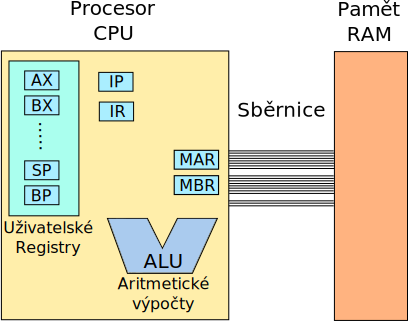
\includegraphics[width=0.5\textwidth]{cpu.pdf}
\end{center}

\end{frame}

\begin{frame}
\frametitle{Paměť}

Paměť si pamatuje data - bajty, slova.

Pokud už znáte nějaký programovací jazyk, tak si ji můžete představit jako pole:\\
\texttt{unsigned char RAM[16 * 1024 * 1024 *1024]; // 16GB RAM}

\bigskip
Z paměti lze číst:\\
\texttt{data = RAM[adresa];}\\
nebo zapisovat:\\
\texttt{RAM[adresa] = data;}

\end{frame}

\section{Boolova algebra}
\begin{frame}
\frametitle{Boolova algebra}

Boolova algebra:
\begin{itemize}
\item Používá pouze dvě hodnoty 0,1
\begin{itemize}
\item 0/1, nebo False/True, nebo nesvítí/svítí, nebo 0V/5V
\end{itemize}
\item Oprace plus (nebo, or)
\begin{itemize}
\item 0+0=0   0+1=1
\item 1+0=1   1+1=1
\end{itemize}
\item Oprace krát (a, and)
\begin{itemize}
\item 0*0=0   0*1=0
\item 1*0=0   1*1=1
\end{itemize}
\item Oprace inverzní prvek - (negace, not)
\begin{itemize}
\item -0 = 1
\item -1 = 0
\end{itemize}
\end{itemize}
\end{frame}


\begin{frame}
\frametitle{Boolova algebra}

Booleova algebra se dá dobře implementovat pomocí tranzistorů (nebudeme zkoušet):

%inkscape ctrl shift Y logic symbols
\end{frame}

\begin{frame}
\frametitle{Boolova algebra}

Rozšířené operace nand, nor, xor a libovolné logické funkce se skládají ze základních operací (or, and not)

X nand Y = not(X and Y)
X nor Y = not(X or Y)
X xor Y = (X or Y) and (not(X and Y)) = (X or Y) and (X nand Y)

Některé funkce lze převést do hradel i efektivněji než přes základní logické funkce or, and, not.
\end{frame}

\begin{frame}
\frametitle{Boolova algebra}

Složitější obvody - složené ze základních operací, stavebních bloků

Příklad
\end{frame}


\begin{frame}
\frametitle{Binární soustava - kvíz}

Kvíz: Jeden vodič reprezentuje jednu hodnotu, buď 0 nebo 1. Jak reprezontovat více čísel, třeba od 0 do 255 (jeden bajt):
\begin{itemize}
\item[A] Jeden vodič má 8 rozdílných úrovní napětí
\item[B] Jeden vodič reprezentuje postupně v čase 8 různých hodnot 0/1
\item[C] Osm vodičů, každý reprezentuje v jeden čas jednu z hodnot 0/1
\item[D] 256 vodičů, pouze jeden má hodnotu 1 ostatní 
\end{itemize}


\end{frame}


\begin{frame}
\frametitle{Binární soustava}

Více bitová čísla - binární soustava
\begin{itemize}
\item 8 až 64 jednobitových paralelních vodičů
\item pořadí vodičů je důležité
\item každý vodič reprezentuje jednu mocninu 2
\item vodič a_{i}, celková hodnota s = \sum_{i=0}^{63} a_{i}*2^{i}
\end{itemize}

\end{frame}

\begin{frame}
\frametitle{Sčítání}

Součet dvou jednobitových čísel:
\begin{tabular}{|r|r|r|}\hline
X & Y & X+Y\\ \hline
0 & 0 & 0\\ \hline
0 & 1 & 1\\ \hline
1 & 0 & 1\\ \hline
1 & 1 & 10\\ \hline
\hline
\end{tabular}

Výsledek součtu může být dvoubitové číslo C - přenos, S - součet.

\texttt{S = X xor Y}\\
\texttt{C = X and Y}

\end{frame}

\begin{frame}
\frametitle{Sčítání}

Pokud sčítáme vícebitová čísla potřebujeme:
\begin{tabular}{|r|r|r|}\hline
C & X & Y & C+X+Y\\ \hline
0 & 0 & 0 & 00\\ \hline
0 & 0 & 1 & 01\\ \hline
0 & 1 & 0 & 01\\ \hline
0 & 1 & 1 & 10\\ \hline
1 & 0 & 0 & 01\\ \hline
1 & 0 & 1 & 10\\ \hline
1 & 1 & 0 & 10\\ \hline
1 & 1 & 1 & 11\\ \hline
\hline
\end{tabular}

Výsledek součtu je opět dvoubitové číslo C_{out} - přenos, S - součet.

\texttt{S_1 = (X xor Y)}\\
\texttt{S = (S_1 xor C)}\\
\texttt{C' = (X and Y)}\\
\texttt{C" = (S_1 and C)}\\
\texttt{C_{out} = C' or C"}

\end{frame}

\begin{frame}
\frametitle{Sčítání}

Ripple carry adder
\end{frame}

\begin{frame}
\frametitle{Sčítání}

Rychlost - Ripple carry adder
\end{frame}

\begin{frame}
\frametitle{Sčítání}

Look ahead adder
\end{frame}

\begin{frame}
\frametitle{Sčítání}

Look ahead adder
\end{frame}

\begin{frame}
\frametitle{Sčítání}

Look ahead adder
\end{frame}

\begin{frame}
\frametitle{Sčítání}

Look ahead adder
\end{frame}

\begin{frame}
\frametitle{Sčítání}

Look ahead adder
\end{frame}

\end{document}

